% - passive and active intrinsic lumped, not individually estimated. (schouten had parameters, mugge threw them away)
% - others do same, specify stiffness and damping on joint level, not really considering stiffness / viscosity muscle. lumped larger system
% - intrinsic, no clear separation joint stiffness and damping (due to friction during movement) and muscle intrinsic properties. 
% - intrinsic short range stiffness (time variant or invariant discussion)


% time variant properties: 
% - thixotropy 
% - muscle fatigue (MVC for checking if fatigue happened) (duration of experiments arbitrary, no real check. MVC after e.g. relaxing tasks could be as high as beginning of experiment because of resting, but fatigue during trials can still be present.

\chapter{Assumptions in joint dynamics system identification}
\label{chap:assumptions}
A lot of different studies have been conducted to identify joint dynamics in the human body. The human neuromuscular system is complex, and the joint dynamics can be modulated by different mechanisms, in literature mainly separated into two components, intrinsic and reflexive feedback. To gain a better understanding in the contribution of these components and to determine the underlying physiology, many different models have been proposed. These models vary in complexity and resemblance to the presumed physiology of the human. A wide variety of assumptions have been introduced in studies to simplify the models, enabling identification of the introduced parameters. In this chapter the most important assumptions made in various studies are listed and compared to each other.

It should be noted that for this comparison the focus is on parametric system identification studies. Although subspace identification methods have shown excellent prediction capabilities and have proven to be very robust to high noise conditions, providing good convergence, these studies were not considered due to the fact that the used structures provide little physiological insight \cite{jalaleddini_subspace_2017}. 

% Non-parametric studies have a tendency to describe (?) merely input output relations, and try to find physiological explanations for observed behaviour. Therefore not that interesting as this is not modelled, and assumptions not taken that strictly.

% \section{General model structure}
% \tred[paragraph about general model structure? information about parallel intrinsic and reflexive pathway. moment arms. ]

% ZHANG
\begin{figure}[t]
    \centering
    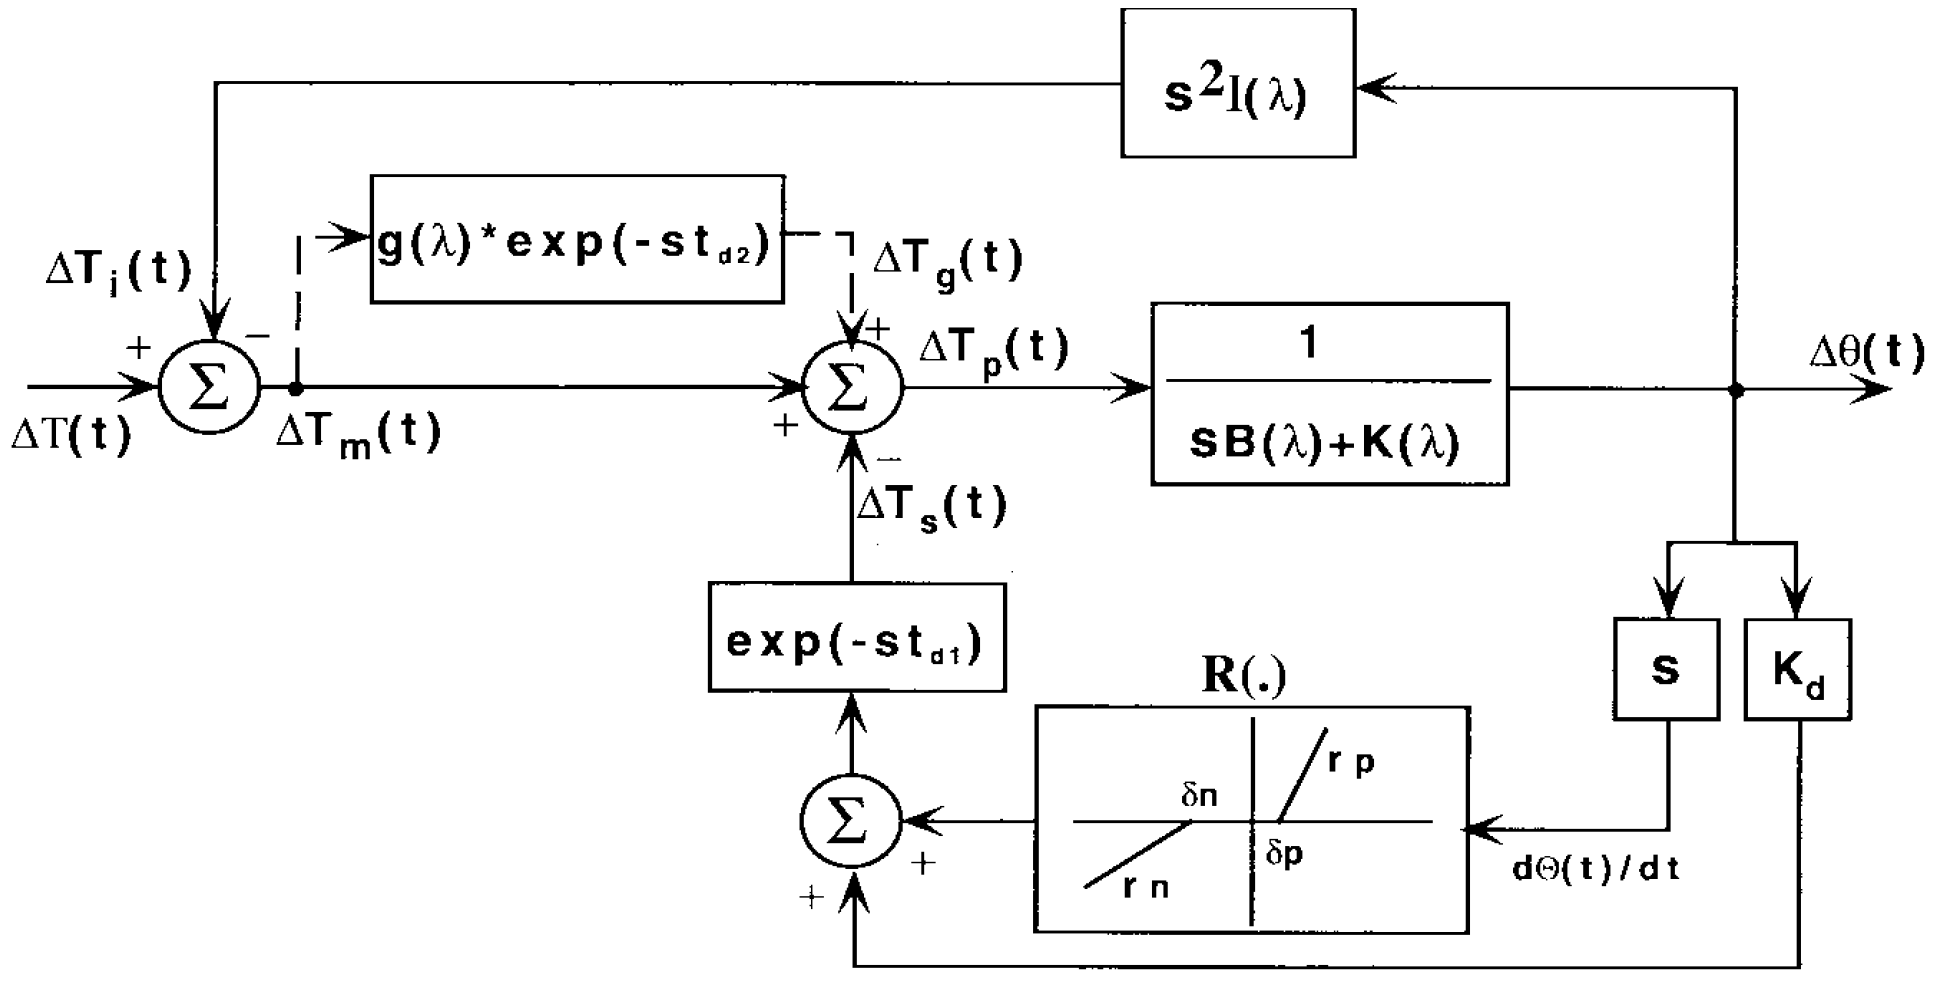
\includegraphics[width=\linewidth]{Figures/models_assumptions/model_zhang_1997.png}
    \caption{The model structure used by \citeauthor{zhang_simultaneous_1997}. System input $\Delta T(t)$ and output $\Delta \theta (t)$ are elbow joint torque and angle deviations respectively. The operating point is denoted by $\lambda$ (i.e. system state). $I(\lambda)$, $B(\lambda)$ and $K(\lambda)$ denote the intrinsic properties limb inertia, joint viscosity and stiffness respectively. The afferent feedback from GTO's is determined by gain $g(\lambda)$ with time delay $t_{d2}$, resulting in torque $\Delta T_g (t)$. The afferent feedback from the MS is separated in a position part with gain $K_d$ and velocity contribution via the asymmetric nonlinearity $R( \bullet )$, finally affected by time delay $t_{d1}$ to result in the torque $\Delta T_s (t)$. Figure adapted from \citet{zhang_simultaneous_1997}.}
    \label{fig:model_zhang_1997}
\end{figure}




\section{Limb muscle structure simplification}
\citeauthor{zhang_simultaneous_1997} modelled the elbow joint \cite{zhang_simultaneous_1997} (see \autoref{fig:model_zhang_1997}), \citeauthor{van_der_helm_identification_2002} and \citeauthor{schouten_nmclab_2008} created a model to identify the shoulder dynamics from the wrist position \cite{van_der_helm_identification_2002, schouten_nmclab_2008} (see \autoref{fig:model_helm_2002} and \ref{fig:model_schouten_2008} respectively) and \citeauthor{mugge_rigorous_2010} modelled the ankle joint \cite{mugge_rigorous_2010}. All these studies lumped the agonist and antagonist muscles into one system. This simplification means that there are no moment arms used. The points of origin or insertion of the individual muscles were not estimated and hence no individual muscle forces were estimated. To account for this, only net joint torques are considered. 

A different approach proposed by \citeauthor{kearney_identification_1997} and later adapted by \citeauthor{mirbagheri_intrinsic_2000} consisted of only modelling the plantar flexor muscles to identify the ankle joint dynamics \cite{kearney_identification_1997, mirbagheri_intrinsic_2000} (see \autoref{fig:model_mirbagheri_2000}). The omission of the dorsiflexor muscles in the model was justified by keeping the experimental conditions such that the dorsiflexor muscles were not activated (validated by EMG measurements). If any activity was measured the data from that trial was discarded. The passive contributions of the dorsiflexor muscles were only apparent in the intrinsic pathway (discussed further in \autoref{sec:ass_intrinsic}). 

Another study by \citeauthor{de_gooijer-van_de_groep_estimation_2016} did use an antagonistic muscle structure, in which the wrist flexor and extensor muscle groups were modelled separately \cite{de_gooijer-van_de_groep_estimation_2016}. This structure required the inclusion of moment arms, which were modelled wrist angle dependent. Since the extensor group consisted of two separate muscles with different tendons (\textit{extensor carpi radialis longus} and \textit{brevis}) and only a combined EMG signal could be measured, the extensor moment arm was taken as the average of the two separate moment arms. 



\section{Muscle-tendon unit modelling}
% \tred[alternative title: measured data to muscle elongation (???)]
The muscle-tendon unit (MTU) is known to have quite complicated dynamics, and the tendon length relative to the muscle fibre length greatly influences the proportion of strain taken up by muscle and tendon \cite{zajac_muscle_1989}. Although these effects are known, many studies take the measured limb position or joint angle proportional to muscle elongation, implying an infinitely stiff tendon. Especially for compliant tendons (large tendon slack length with respect to  optimal muscle fibre length, e.g. Achilles tendon of plantar flexors) significant MTU interaction can lead to a distorted estimation of the force length curve \cite{zajac_muscle_1989}. 

\citeauthor{zhang_simultaneous_1997} acknowledged that the tendon in the MTU plays a significant role for abrupt change in muscle length, which they accounted by using small amplitude perturbations \cite{zhang_simultaneous_1997}. As a consequence, the joint angle was taken proportional to muscle elongation in the parameter estimation. \citeauthor{mirbagheri_intrinsic_2000} also took the ankle rotation proportional to the muscle elongation, i.e. not considering MTU dynamics, though abrupt changes in muscle length were present during their experiments \cite{mirbagheri_intrinsic_2000}. Similarly, \citeauthor{de_gooijer-van_de_groep_estimation_2016} took the wrist angle proportional to muscle elongation (corrected angle dependent moment arm), hence no MTU interaction was modelled \cite{de_gooijer-van_de_groep_estimation_2016}. 

In the study of \citeauthor{van_der_helm_identification_2002} the wrist position was taken proportional to muscle stretch, and tendon stretch was not considered. There was however a viscoelastic contact model considered to link the measured handle position to the hand position, representing the displacement of skin and movement of fingers \cite{van_der_helm_identification_2002}. This contact model was also employed by \citeauthor{schouten_nmclab_2008} for the wrist and \citeauthor{mugge_rigorous_2010} for the foot, to obtain the estimated wrist position and ankle angle respectively \cite{schouten_nmclab_2008,mugge_rigorous_2010}. These two studies did however consider separate muscle and tendon elongation. The force in tendon and muscle was assumed equal (connected in series), and consequently part of the joint translation or rotation was accounted by the tendon with estimated stiffness $k_\text{tendon}$. The muscle contractile element was represented by a linearized Hill model. 



% MIRBAGHERI
\begin{figure}[t]
    \centering
    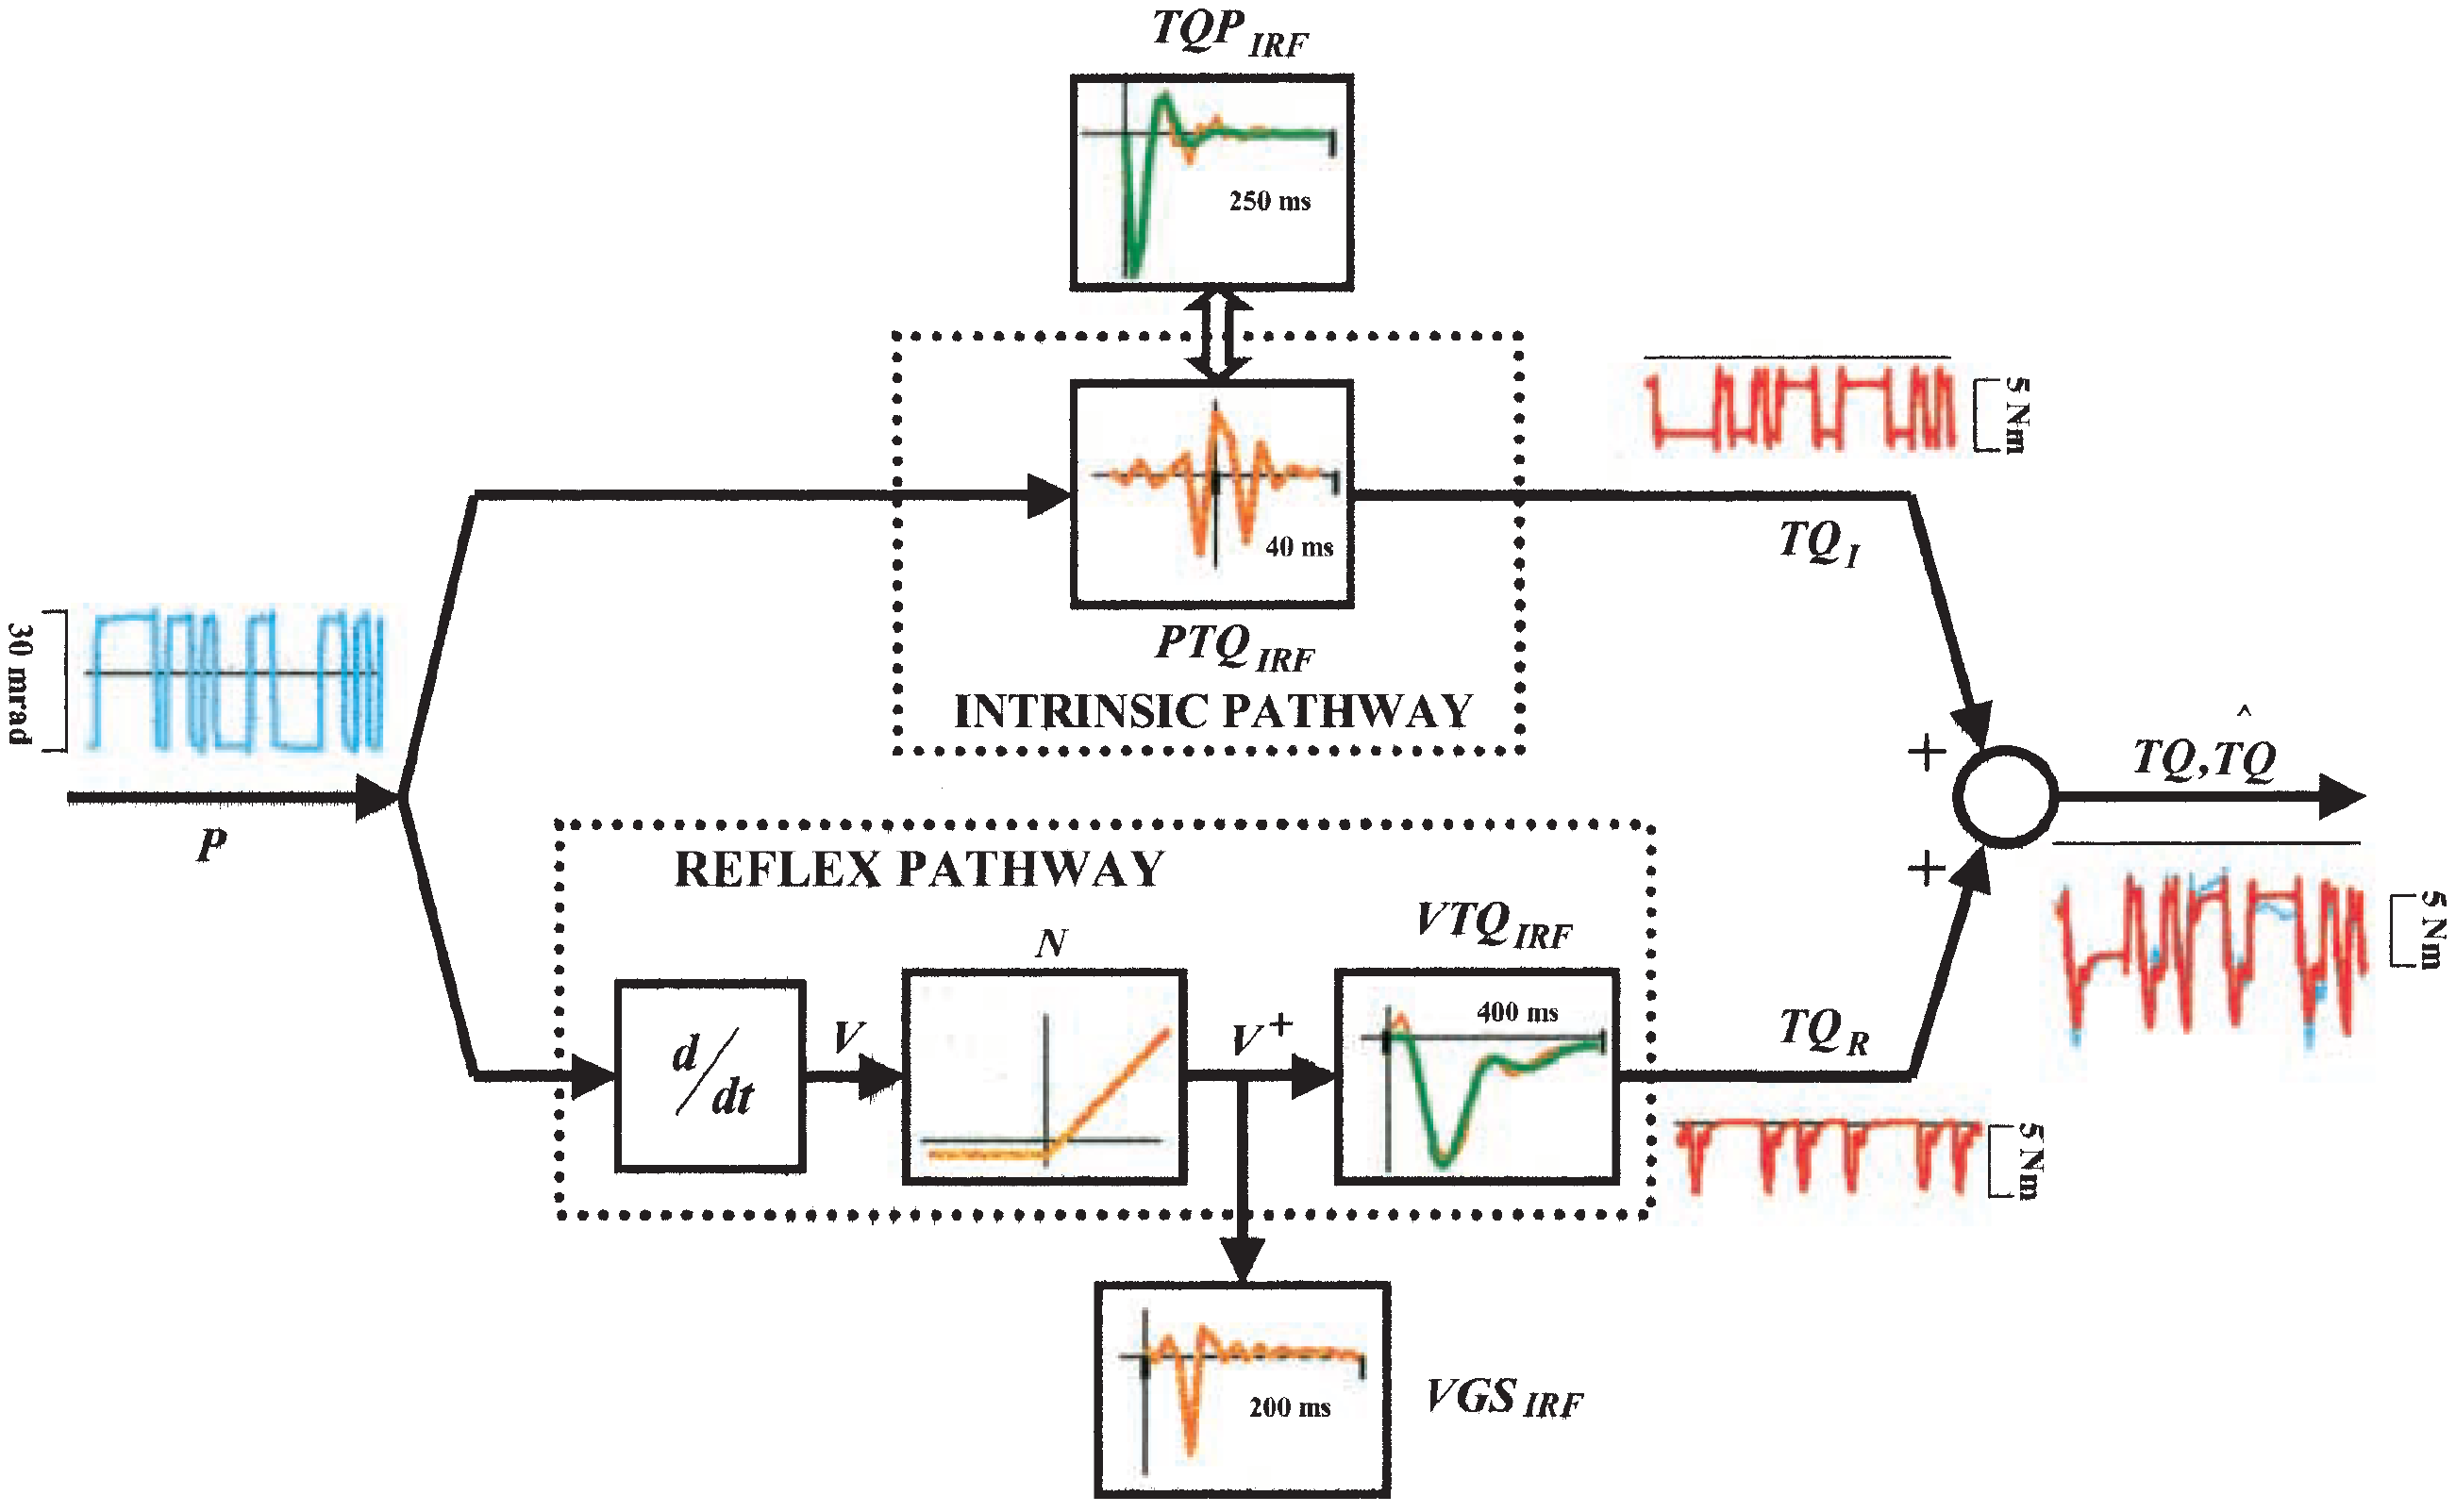
\includegraphics[width=\linewidth]{Figures/models_assumptions/model_mirbagheri_2000.png}
    \caption{Model structure of \citeauthor{mirbagheri_intrinsic_2000}, top pathway represents the intrinsic contribution, modelled by a second order spring-damper system with $I$, $B$ and $K$. The bottom pathway represents afferent feedback, only mediated by velocity feedback. The velocity is passed through a static nonlinearity $N$, closely resembled by a half-wave rectifier, resulting in only positive velocity $V^+$. This is used as activation signal for the reflex stiffness dynamics, $VTQ_{IRF}$, which comprises  a third order model with a time delay. Figure adapted from \citet{mirbagheri_intrinsic_2000}.}
    \label{fig:model_mirbagheri_2000}
\end{figure}



\section{Muscle activation dynamics}
\label{sec:muscle_act_dyn}
Upon application of an neural activation signal to the muscle, it takes some time for the muscle to buildup force, characterised by the muscle activation dynamics. In the considered studies different systems are used to describe these dynamics, though there is not as much variation as in the other aspects of the neuromuscular system. 

\citeauthor{zhang_simultaneous_1997} did not model any separate activation dynamics, but simplified this process by incorporating it in the modelled time delays for the afferent feedback (discussed further in \autoref{sec:ass_afferent}) \cite{zhang_simultaneous_1997}. In \citeauthor{van_der_helm_identification_2002}, the activation dynamics were modelled as a first order low-pass filter \cite{van_der_helm_identification_2002}. 

A more frequently used representation of the activation dynamics is a second order low-pass filter \cite{schouten_nmclab_2008, mugge_rigorous_2010}. \citeauthor{mirbagheri_intrinsic_2000} also used second order low-pass activation dynamics, but did not find a good fit in previous work, and therefore included a first order pole in the model \cite{mirbagheri_intrinsic_2000, mirbagheri_parametric_1995}. The entire model by \citeauthor{mirbagheri_intrinsic_2000} was similar to the model structure proposed by \citeauthor{kearney_identification_1997}, except for this additional pole. In general, it is assumed that the activation dynamics only affect the afferent feedback path, since the intrinsic properties are assumed constant and instantaneous during trials (see \autoref{sec:ass_intrinsic}). 

The model of \citeauthor{de_gooijer-van_de_groep_estimation_2016} also employed second order filter activation dynamics and used it to relate measured EMG activity to the active state of the muscle \cite{de_gooijer-van_de_groep_estimation_2016}. The active state (in combination with muscle length and velocity) was used to determine the force in the muscle using a Hill-type muscle model. 


% HELM
\begin{figure}[t]
    \centering
    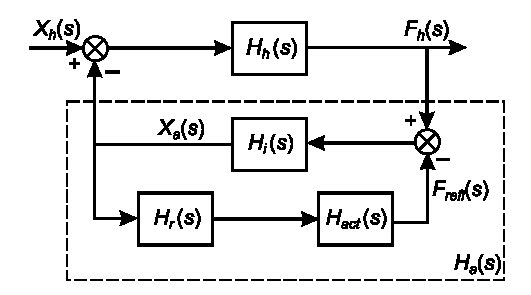
\includegraphics[width=0.6\linewidth]{Figures/models_assumptions/model_helm_2002.pdf}
    \caption{Linear model used by \citeauthor{van_der_helm_identification_2002}, the handle position $X_h(s)$ is the input of the model. From the difference in handle position and arm position, the handle force $F_h(s)$ is estimated (model output), by means of a viscoelastic hand-grip contact model $H_h(s)$. This handle force is used to determine the arm position $X_a(s)$. The arm position is then used to determine the reflexive contribution via $H_r(s)$, which comprises MS position and velocity feedback and a time delay. The reflexive contribution is then affected by the muscle activation dynamics $H_\text{act}(s)$ (first order low-pass filter), to result in the reflexive force contribution $F_\text{refl}(s)$. Figure adapted from \citet{van_der_helm_identification_2002}.}
    \label{fig:model_helm_2002}
\end{figure}




\section{Afferent feedback} \label{sec:ass_afferent}
Afferent feedback (also referred to as reflexive feedback) is considered as the muscle activity that results from feedback of the sensory organs in the muscles. In comparison to assumptions made in other aspects of the system identification (which for the most part can be considered as simplifications for parameter estimation), the modelling of the afferent feedback is mostly influenced by the fact that there is no consensus about the origin of the different observed reflexes. Afferent feedback is considered energy efficient, since it only provokes muscle activity in response to a perturbation. 

The two known receptor organs described in physiological studies are the muscle spindles (MS) and Golgi tendon organs (GTO). The muscle spindles are located in the muscle belly, parallel to the muscle fibres and are presumed to be sensitive to fibre stretch (also referred to as position) and velocity. It is believed that both the fibre stretch and velocity information is transmitted through the Ia afferent nerve fibre to the $\alpha$-motoneuron, and only the fibre stretch through the II afferent nerve fibre. Two efferent $\gamma$ neurons are believed to set the sensitivity of the MS, one dynamic mostly influencing the sensitivity of the Ia afferent, and one static mostly influencing the II afferent \cite{mileusnic_mathematical_2006}. Furthermore, it is believed that the muscle spindle has an asymmetric response, with the Ia afferent mostly sensitive to eccentric velocity, and the II afferent mainly sensitive to elongation with respec to the resting length \cite{burke_muscle_1978}. 

The other receptor, the Golgi tendon organ, is located exclusively at the muscle-tendon or muscle-aponeu- rosis junction \cite{jami_golgi_1992}, hence in series with the muscle fibres. When the MTU elongates, the GTOs are compressed, and they will start firing through the afferent Ib nerve fibre. The stretch in the tendon is a measure for the force in the muscle, since muscle and tendon are in series. It is shown however that the GTO is more sensitive to active muscle contraction than to passive muscle stretch \cite{houk_responses_1967}.

In the model by \citeauthor{de_gooijer-van_de_groep_estimation_2016} no proprioceptors were modelled, thus no attempt was made identify the origin of the reflex activity since it was out of their scope \cite{de_gooijer-van_de_groep_estimation_2016}. The model was a variation on the model of \citeauthor{de_vlugt_relation_2010}, where it was explained that the modelling of proprioception was not required since EMG activity was used directly to estimate the muscle torques \cite{de_vlugt_relation_2010}. Because of the used ramp and hold (RaH) perturbations in combination with the task description to completely relax, it was expected that only reflexive activity was evoked. The absence of voluntary contractions in the EMG signal could not be validated. 


% MS feedback has been described as asymmetric \cite{terjung_neural_2011} 
% The modelling of afferent feedback varies the most across the considered studies, and the underlying mechanism is 

\subsection{Receptor modelling}
The modelling of the two receptors varies a lot between the studies (see overview in \autoref{tab:overview_assumptions}, column afferent feedback). \citeauthor{mirbagheri_intrinsic_2000} considered only velocity feedback, presumably arising from MS feedback though not explicitly written \cite{mirbagheri_intrinsic_2000}. The measured angle was differentiated and the resulting angular velocity of the ankle was provided to a static nonlinear element, a half wave rectifier. As a consequence, reflexive feedback was only evoked by eccentric velocity of the plantar flexor muscles, corresponding to the unidirectional sensitivity of the stretch reflex \cite{kearney_system_1983}. The output of the nonlinearity was normalised, and thus only corresponds to the activation caused by the velocity. No muscle fibre length or muscle force feedback was considered. The model used by \citeauthor{mirbagheri_intrinsic_2000} was first introduced by \citeauthor{kearney_identification_1997}, and slightly adapted, but the receptor modelling remained unchanged. 
% \tred[discuss gain IRF? or in integration] 

Initially, \citeauthor{zhang_simultaneous_1997} did model both MS and GTO feedback. The MS feedback was separated in a velocity and position component, of which the former was modelled by two half-wave rectifiers (one for concentric and one for eccentric muscle velocity) \cite{zhang_simultaneous_1997}. These were modelled asymmetrically, since the response of the MS to positive and negative velocity was assumed different \cite{houk_neural_1981}. Each side of the half-wave rectifiers was specified by a slope and a threshold, resulting in an asymmetric dead-zone. The MS position feedback was taken as a simple gain, hence not asymmetric. In the initial model force (GTO) feedback was incorporated, also represented by a gain. However, in a simplified version of the model for the parameter estimation, GTO feedback was omitted, as well as the dead-zone for the velocity feedback. %All parameters were taken dependent on the operating state, among which the mean joint angle, mean background torque and perturbation properties. 

The model of \citeauthor{van_der_helm_identification_2002} included position and velocity feedback, representing MS feedback, but no force feedback was used in the model \cite{van_der_helm_identification_2002}. It was later mentioned that the inclusion of force feedback in the model yielded very small force reflex gains or bad convergence of the model, which the authors ascribed to negligible force feedback under the presented experimental conditions. The position and velocity feedback were described by separate gains, $k_p$ and $k_v$ respectively. 

The model introduced by \citeauthor{schouten_nmclab_2008} was \tred[the first] to incorporate both GTO and MS feedback and estimate these parameters \cite{schouten_nmclab_2008}. GTO feedback was modelled as a gain $k_f$, and was activated by the estimated force in the MTU. Since GTO feedback is mostly associated with inhibitory effects, a positive gain was considered inhibitory and a negative gain excitatory. The MS feedback was similar to \citeauthor{van_der_helm_identification_2002} modelled by gains for the position, $k_p$, and velocity, $k_v$. For the MS, positive gains were associated with excitatory effects, and negative with inhibitory. In addition, since some studies suggested the MS was also sensitive to fibre acceleration, an additional acceleration gain, $k_a$, was modelled. However this gain was later set to zero without explanation. The study by \citeauthor{mugge_rigorous_2010} used the same model as \citeauthor{schouten_nmclab_2008}, but removed the acceleration gain \cite{mugge_rigorous_2010}.

In all studies where MS feedback consisted of both position and velocity feedback, these were separated completely, unlike the presumed underlying physiology where the Ia afferent is believed to be sensitive to both and the II afferent to merely position \cite{van_der_helm_identification_2002, schouten_nmclab_2008, mugge_rigorous_2010}. Furthermore, although the unidirectional (nonlinear) properties of the MS were acknowledged in these studies, these were not modelled. The used structure, flexor and extensor lumped, did not allow for this. But as a result the inhibitory and excitatory effects of MS feedback are equal in size for equal valued $k_p$ and $k_v$ with different signs. This is not in correspondence with reality, where the flexor and extensor muscles often cannot deliver an equal amount of force (see e.g. \cite{winters_analysis_1985}). 


% SCHOUTEN
\begin{figure}[t]
    \centering
    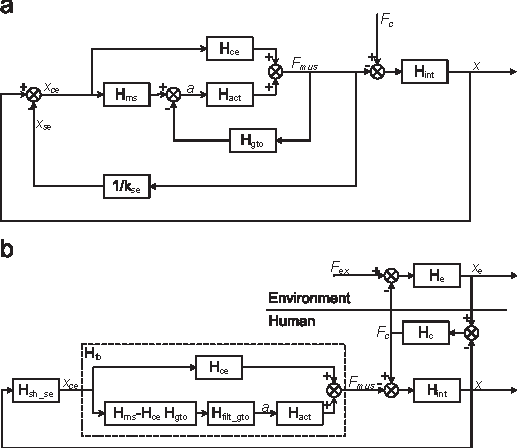
\includegraphics[width=.8\linewidth]{Figures/models_assumptions/model_schouten_2008.pdf}
    \caption{Model structure used by \citeauthor{schouten_nmclab_2008} to identify shoulder joint dynamics. \textbf{(a):} Intrinsic dynamics due to tonic contraction are described in $H_\text{ce}$. Parallel to this, the reflexive contribution is obtained from the MS feedback ($H_\text{ms}$) excited by length ($x_\text{ce}$) and lengthening velocity and GTO feedback ($H_\text{gto}$) excited by muscle force $F_\text{mus}$. \textbf{(b):} Human in combination with the environment, including contact ($H_\text{c}$) and robotic manipulator dynamics ($H_\text{e}$). The difference in contact and muscle force determine the force affected by the inertia ($H_\text{int}$) of the limb. The model structure used by \citet{mugge_rigorous_2010} was very similar, with some differences in additional external signals (e.g. neural activation additional to voluntary co-contraction). Figure adapted from \citet{schouten_nmclab_2008}. }
  \label{fig:model_schouten_2008}
\end{figure}


% SCHOUTEN AND MUGGE
% \begin{figure}[t]
% % \centering
% \begin{minipage}[t]{.53\textwidth}
%   \centering
%   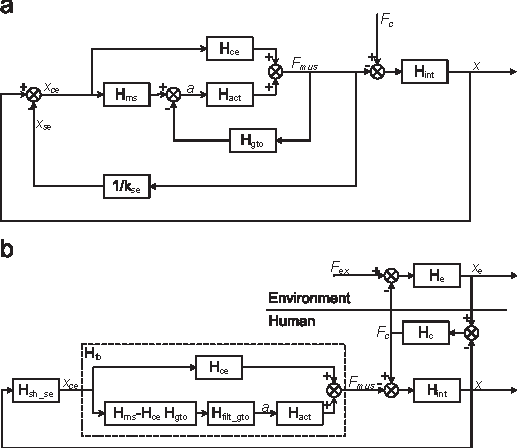
\includegraphics[width=\linewidth]{Figures/models_assumptions/model_schouten_2008.pdf}
%   \captionof{figure}{Model structure used by \citeauthor{schouten_nmclab_2008} to identify shoulder joint dynamics. \textbf{(a):} Intrinsic dynamics due to tonic contraction are described in $H_\text{ce}$. Parallel to this, the reflexive contribution is obtained from the MS feedback ($H_\text{ms}$) excited by length ($x_\text{ce}$) and theningleng velocity and GTO feedback ($H_\text{gto}$) excited by muscle force $F_\text{mus}$. \textbf{(b):} Human in combination with the environment, including contact ($H_\text{c}$) and robotic manipulator dynamics ($H_\text{e}$). The difference in contact and muscle force determine the force affected by the inertia ($H_\text{int}$) of the limb. Figure adapted from \citet{schouten_nmclab_2008}. }
%   \label{fig:model_schouten_2008}
% \end{minipage} $\quad$
% \begin{minipage}[t]{.43\textwidth}
%   \centering
%     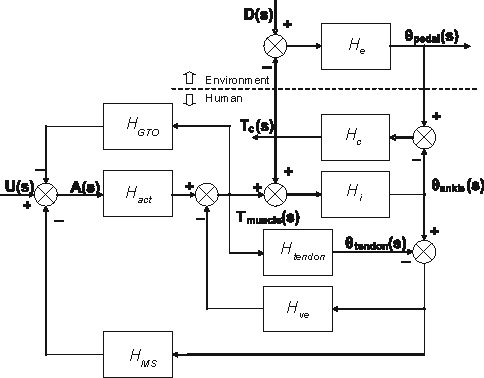
\includegraphics[width=\linewidth]{Figures/models_assumptions/model_mugge_2010.pdf}
%     \caption{Model structure used by \citeauthor{mugge_rigorous_2010}, derived from \cite{schouten_nmclab_2008}.  Figure adapted from \citet{mugge_rigorous_2010}.}
%     \label{fig:model_mugge_2010}
% \end{minipage}
% \end{figure}


% \begin{figure}[t]
%     \centering
%     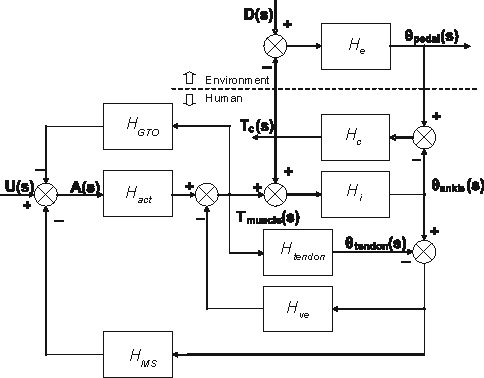
\includegraphics[width=\linewidth]{Figures/models_assumptions/model_mugge_2010.pdf}
%     \caption{Model structure used by \citeauthor{mugge_rigorous_2010}, derived from \cite{schouten_nmclab_2008}. Figure adapted from \citet{mugge_rigorous_2010}.}
%   \label{fig:model_mugge_2010}
% \end{figure}



\subsection{Time delays}
\label{sec:ass_afferent_delay}
Afferent feedback has a substantial time delay from detection of the receptor organs to muscle action, caused by travel time from the receptors to the motoneurons via the afferent nerve fibre, processing of the detected changes and travel time of the motor command via the efferent nerve fibre. The neural travel time limits the ability of reflexive feedback to be effective for high frequency perturbations. The modelling of the delays shows some variation across the considered studies. In all studies the afferent, processing and efferent delays are lumped into one for simplicity, but the variation lies in the separation of MS and GTO feedback delay.

\citeauthor{zhang_simultaneous_1997} modelled the GTO and MS delay as separate two variables \cite{zhang_simultaneous_1997}. Although the GTO feedback was later omitted, it was assumed that the GTO delay was larger due to the involvement of interneurons. To estimate the time delay for MS feedback, a tendon tapping experiment was performed separately. The modelled time delay included the muscle activation dynamics (as discussed in \autoref{sec:muscle_act_dyn}), and thus the delay was taken as the time between the moment of tendon tapping and the onset of reflex torque. \citeauthor{mirbagheri_intrinsic_2000} and \citeauthor{van_der_helm_identification_2002} did not consider GTO delay, hence the modelled delay only represents MS delay \cite{mirbagheri_intrinsic_2000, van_der_helm_identification_2002}. \citeauthor{schouten_nmclab_2008} used the same value for the time delay for both GTO and MS feedback \cite{schouten_nmclab_2008}. Dynamics of the $\alpha$-motoneuron pool at the spinal cord, integrating all the afferent feedback, were assumed much faster than the other dynamics in the loop, and was not modelled individually. \citeauthor{mugge_rigorous_2010} used mostly the same model, but made a slight variation in the time delays by considering separate parameters for GTO and MS feedback \cite{mugge_rigorous_2010}. The reported parameter for MS delay was longer than GTO delay, contradicting the assumption of \citeauthor{zhang_simultaneous_1997}. 

All these modelled time delays are only able to capture the short-latency reflex (SLR), which is a monosynaptic reflex. Other more coordinated reflexes as the medium- and long-latency reflex (MLR and LLR respectively), presumably more spinal levels are involved, hence longer neural travel time and longer integration time. This makes it a lot harder to model, involves a lot more uncertainty, and therefore these longer latency reflexes are often omitted for simplification of the models. \citeauthor{mugge_rigorous_2010} did try to substitute the SLR for the LLR by changing the boundaries for the delay parameters in the parameter estimation \cite{mugge_rigorous_2010}. This yielded worse fits compared to the SLR boundaries. In reality, presumably a combination of SLR, MLR and LLR is present, but there have been no attempts to incorporate this combination in parametric system identification studies. 

\subsection{Sensitivity to afferent feedback}
In the central nervous system (CNS), there are mechanisms to set the sensitivity of the muscle spindles, allowing the CNS to change the reflex response to detected length and velocity information. According to the `fusimotor set' hypothesis, this is is done through two efferents from the $\gamma$-motoneurons, the static and dynamic efferents ($\gamma_s$ and $\gamma_d$ respectively) \cite{prochazka_fusimotor_1985}. These are assumed to set the sensitivity of the Ia and II afferents independently, and are set consistently for certain types of movements. A similar mechanism to adapt the sensitivity for force feedback (Ib afferent) does not exist. Moreover, a static and linear relation between muscle force and afferent activity is found \cite{crago_sampling_1982}. The mechanism to change the sensitivity to muscle force feedback are set in the CNS, e.g. presynaptic inhibition, by changing the sensitivity of the Ib afferent receiving neuron. This shows that the CNS has many mechanisms to change the sensitivity of the different types of afferent feedback and thus modulate the $\alpha$-motoneuron activity. 

The gains for the afferent feedback in the considered studies were all modelled constant for each presented condition. The $\gamma_s$ and $\gamma_d$ were assumed constant per task type in \cite{van_der_helm_identification_2002, schouten_nmclab_2008, mugge_rigorous_2010}, resulting in static $k_p$ and $k_v$ gains, per task movement type. If force feedback was modelled this was also modelled by a constant gain, again dependent on the type of movement. The type of movement was controlled by specifying a tasks, and varying the bandwidth of the presented perturbations. Hence, for each condition the different parameters were estimated. The other studies also took the gains for the modelled reflexive feedback constant during a movement type, but estimated it dependent on  e.g. the presented background torque, joint configuration and perturbation properties \cite{zhang_simultaneous_1997, mirbagheri_intrinsic_2000}. 

% Gains afferent feedback
% All studies including afferent feedback organs (Helm, Schouten, Mugge, …) : Gamma static and dynamic and GTO gain modelled constant (time invariant), only dependent on task. 
% Mirbagheri et al 2000; determined IRFs per condition, and in condition constant can be compared to constant gain per condition
% Zhang Rymer 1997; same, nonlinearity parameters (slope + and -) and pos gain determined per background torque. (~ time invariant for task) 


\section{Linear versus nonlinear}
Although it is known that the human body behaves highly nonlinear, many studies used linear modelling techniques \cite{van_der_helm_identification_2002, schouten_nmclab_2008, mugge_rigorous_2010}. As a consequence, small perturbation signals have to be used, to disturb the system near the operating point that is being identified. When large amplitude (or high velocity) perturbations are applied, the nonlinearities in the system are excited, and the linear model will not be able to explain the measured output of the signal. \citeauthor{schouten_nmclab_2008} and \citeauthor{mugge_rigorous_2010} employed a Hill model for the dependency of muscle length and velocity on the muscle force, which had to be linearized first \cite{schouten_nmclab_2008, mugge_rigorous_2010}.

%\citeauthor{zhang_simultaneous_1997} and \citeauthor{mirbagheri_intrinsic_2000}
The studies that did include nonlinearities in their model (for the MS feedback) still used low amplitude perturbation signals (\citeauthor{zhang_simultaneous_1997} standard deviation on amplitude 1.5 deg \cite{zhang_simultaneous_1997}, \citeauthor{mirbagheri_intrinsic_2000} amplitude jumps of approx. 1.7 deg \cite{mirbagheri_intrinsic_2000}). The used perturbation signal is typically continuous, having frequency content equally distributed across a specified bandwidth \cite{zhang_simultaneous_1997, van_der_helm_identification_2002, schouten_nmclab_2008, mugge_sensory_2009}. In contrast, \citeauthor{mirbagheri_intrinsic_2000} used pseudorandom binary sequence (PRBS) signals, jumping at random time instances to another peak value. In these sequences, the maximum velocity in the ankle was approx. 11 deg/s \cite{mirbagheri_intrinsic_2000}. A clear difference in the PRBS trials compared to continuous trials, is that in PRBS the velocity distribution is a lot smaller, while still exiting a broad frequency range. On the other hand, the power at the different frequencies is not as equally distributed as in continuous perturbation signals. 

The ramp and hold (RaH) perturbations used by \citeauthor{de_gooijer-van_de_groep_estimation_2016} were high in amplitude, i.e. over the full range of motion (RoM) of the wrist joint. Furthermore, the movement over the complete RoM was imposed in \SI{1}{\second}, resulting in high angular velocities. Therefore, a nonlinear model was used to capture the nonlinear joint physiology. Forces were estimated with nonlinear force-length and force-velocity curves (adapted from \cite{thelen_adjustment_2003}), and the force in the muscle parallel elastic element was nonlinear. 



% XXX
% \section{Time variant versus time invariant}

% \subsection{EMG proportional to muscle force}

% \subsection{Muscle thixotropy}
% XXX




\section{Intrinsic feedback} \label{sec:ass_intrinsic}
Intrinsic properties are considered as the the mechanical properties of the joint, passive tissue, and active muscle fibres. The main source of intrinsic feedback is seen as the viscoelastic properties of the muscles, determined by the force-length and force-velocity characteristics of the muscle \cite{winter_biomechanics_1988}. The viscoelastic properties can be increased by muscle co-contraction. The major difference between intrinsic and reflexive feedback is that intrinsic feedback is instantaneous, where reflexive feedback is characterised by delays (as discussed in \autoref{sec:ass_afferent_delay}). The instantaneous property of intrinsic feedback makes it very effective for rejecting perturbations at higher frequencies, at cost of greater energy consumption due to the need for a high degree of muscle co-contraction. The modelling of intrinsic feedback shows some variation. 

% 
\citeauthor{zhang_simultaneous_1997} described the intrinsic feedback by a second order spring-damper system, where the inertia included the contribution of the limb and a wrist attachment \cite{zhang_simultaneous_1997}. A separate experiment to estimate the inertia was performed, in which the subjects were asked to fully relax their arm during perturbation. The stiffness $k$ and damping $b$ were taken dependent on the operating point.
 
\citeauthor{mirbagheri_intrinsic_2000} also modelled the intrinsic properties as a second order spring-damper model, completely parallel to the afferent feedback \cite{mirbagheri_intrinsic_2000}. The stiffness $k$ and damping $b$ describe the dynamic viscoelastic properties of the muscle, and the inertia $I$ the static properties of both the limb and boot worn during the experiment. Since the intrinsic pathway was completely parallel to the afferent path, the reflexive forces were not affected by the inertia of the limb and boot. However, due to the model parametrisation, the effects of inertia on reflexive feedback could be hidden in some of the parameters describing the activation dynamics (not all parameters have a direct physiological meaning). To make sure that the intrinsic properties were not contaminated by reflex effects, the length of the IRF representing intrinsic feedback was constrained to be less than the delay associated with afferent feedback, ca. \SI{40}{\milli\second}. 

In the model of \citeauthor{van_der_helm_identification_2002}, the intrinsic properties were also described by a second order spring-damper system \cite{van_der_helm_identification_2002}. No separate parallel pathway for intrinsic feedback exists, hence reflexive feedback is affected by the stiffness, damping (viscosity) and inertia of the joint. The stiffness and damping parameters increase with the level of (co-)contraction. 

\citeauthor{schouten_nmclab_2008} and \citeauthor{mugge_rigorous_2010} take inertia of the limb separate, and model no separate passive viscoelastic properties of the joint \cite{schouten_nmclab_2008, mugge_rigorous_2010}. The active viscoelastic intrinsic properties ($k$ and $b$) due to (co-)contraction (tonic contraction) are modelled parallel to the afferent feedback, not affected by the activation dynamics (i.e. instantaneous force) and dependent on both the operating point and task type of a trial. The resulting intrinsic contribution (tonic) is then summed with the afferent contribution (phasic), and the sum of both is affected by the inertia of the limb.

Since the RaH perturbations used by \citeauthor{de_gooijer-van_de_groep_estimation_2016} were assumed to only evoke reflexive activity, the intrinsic properties were not affected by voluntary (co-)contraction \cite{de_gooijer-van_de_groep_estimation_2016}. The intrinsic contribution to movement was modelled by the passive elastic element parallel to the contractile element in the Hill-type muscle model. The elastic element possibly also contained contribution from the tendon stiffness and joint resistance. This elastic force was assumed to decrease, due to relaxation in the muscle connective tissue, modelled by a first order filter. This was previously modelled by \citeauthor{de_vlugt_relation_2010} as a viscous damper, more similar to the other studies \cite{de_vlugt_relation_2010}. Inertia was also estimated, consisting of the wrist, hand and manipulator handle. 

In none of the studies additional supra spinal commands were considered. The supra spinal commands were assumed constant depending on task type, and were modelled by viscoelastic parameters of the active co-contracted muscles. The level of co-contraction was taken movement type (or task) dependent in all the studies, and hence the stiffness and viscosity parameters were taken constant during the trials. The inertia was in some studies taken condition independent, and thus could be kept constant during the parameter estimation \cite{zhang_simultaneous_1997, van_der_helm_identification_2002, mugge_sensory_2009}.


% \subsection{viscoelasticity parameters independent}
In all studies, the intrinsic viscoelastic parameters (stiffness $k$ and viscosity $b$) were estimated independent. However, in reality there is significant parameter interplay, due to the underlying physiological mechanisms. This relation has been described by using e.g. a Voigt model, and the viscoelastic properties have been estimated using shear wave spectroscopy \cite{gennisson_viscoelastic_2010}. 
% XXX

% \subsection{Short range stiffness}








% ===========================================================================
\section{Implication of assumptions}
% NOTE: all assumptions are closelty interconnected, hence a clear separation is hard to do. Two main assumptions to which the others are closely related will be discussed, and the implications thereof. 
There is a wide variety in modelling of the neuromuscular system across the studies, based on various assumptions. The wide variety in modelling approaches shows that not all studies have the same goal. Where \cite{kearney_identification_1997, mirbagheri_intrinsic_2000, de_gooijer-van_de_groep_estimation_2016, jalaleddini_subspace_2017} used a model with as little as possible \textit{a priori} knowledge, other studies attempted to build (simplified) models based on the current believes about the human physiology involved with reflexes and movement \cite{zhang_simultaneous_1997, van_der_helm_identification_2002, schouten_nmclab_2008, mugge_rigorous_2010}. The former can be seen as more phenomenological studies, which can be used to determine characteristic differences between populations, but are not as informative as the latter, where the goal is to improve the understanding of the underlying physiology and relate changes in the physiologic state to the observed behaviour. Hence, the various identified assumptions all lead to some implications for system identification of the joint dynamics, and have a great influence on what exactly can be learned from the experiment and model. Since the assumptions and their implications are for the most part closely related, these cannot be clearly separated. Therefore, the implications will be discussed based on two main assumptions, relating to muscle-tendon interaction and lumping of muscles. 


\subsection{Muscle-tendon interaction}
A number of system identification studies did not consider muscle-tendon interaction, and consequently related joint ankle or position directly to muscle elongation \cite{zhang_simultaneous_1997, kearney_identification_1997, mirbagheri_intrinsic_2000, van_der_helm_identification_2002, de_gooijer-van_de_groep_estimation_2016}. When it is assumed that no MTU interaction occurs, this directly implies an infinitely stiff tendon. Especially for compliant tendons, such as the Achilles tendon connected to the plantar flexors in the lower leg, significant MTU interaction can be expected, which can lead to a distorted estimation of the muscle elongation. This has consequences for the separation of intrinsic and reflexive contributions to the movement. 

Not considering MTU interaction can lead to a distorted estimation of muscle elongation and subsequently distortion in the estimated contribution of intrinsic properties to movement. In general, a simple spring-damper system consisting of two parameters is used to describe the intrinsic properties of all muscles, passive tissue, tendons and joint resistance. Since these components do not all displace the same amount due to MTU interaction and different moment arms, the estimation of intrinsic properties is distorted (further discussed in \autoref{sec:rem_lumping-muscle}). 

Likewise, the distorted estimation of muscle elongation has implications on the degree of proprioceptive afferent activity leading to modulation of reflexes. The muscle spindles are sensitive to muscle elongation and lengthening velocity, which in case of an infinitely stiff tendon would be overestimated, since all the elongation is ascribed to the muscle. Some studies considered either position or velocity feedback, which has proven to result in models with reasonable \textit{variance accounted for} (VAF), but presumably leads to further overestimation of a single component to reflex modulation \cite{maas_is_2009}. Furthermore, all of the studies that did not model muscle-tendon interaction also omitted the Golgi tendon organ (i.e. force) afferent feedback. Omission of force feedback can further lead to overestimation of the modelled reflexive mechanism. The choice of proprioceptive receptor modelling does not seem to have a large influence on the prediction capabilities of the model (in terms of VAF), but do not necessarily resemble the physiology behind reflex modulation. 
% point about tendon in series, stiffness lot higher than muscle in passive state, hence due to 1/keq = 1/k1 + 1/k2 minor contribution. However, for fast movements, this is not the case.

Especially the omission of GTO force feedback contradicts findings reported by the group of Sinkjaer. Af Klint et al. found strong support for contribution of GTO feedback in addition to MS feedback in adaptations to ground irregularities during locomotion \cite{klint_afferent_2009}. However, the effect of GTO and MS feedback during locomotion appeared to be stance phase dependent, where respectively mid-stance MS feedback and late-stance GTO feedback was thought to be dominant \cite{grey_positive_2007, af_klint_sudden_2009}. This emphasises the need for additional measurement data, enabling further isolation of afferent activity during other motor tasks (i.e. balance, force, position tasks). 

% \tred[expected GTO feedback? Sinkjaer, af Klint??] \textcolor{red}{\lipsum[1]}
% - when not considered, GTO omitted. no physiological basis refl modulation
%     - expected role is substantial (sinkjaer, klint... ??)
% - Wrong estimation leads to wrong activation signal when considering afferent feedback


\subsection{Lumping muscle structure}
\label{sec:rem_lumping-muscle}
A very common simplification of the neuromuscular model is lumping of antagonistic muscle groups \cite{zhang_simultaneous_1997, van_der_helm_identification_2002, schouten_nmclab_2008, mugge_rigorous_2010}. This has as advantage that the model can be defined by less parameters compared to an antagonistic model (e.g. \cite{de_gooijer-van_de_groep_estimation_2016}). No moment arms for MTUs have to be estimated or averaged over multiple MTUs for the same function (i.e. flexion versus extension). Furthermore, the intrinsic properties (i.e. inertia, stiffness and damping) of limb, joint resistance, tendon, passive and active muscle tissue can all be lumped into a minimum of three parameters. The lumping of muscle groups with different function does however also have disadvantages when the intrinsic and reflexive effects on movements are under analysis. 

% - afferent inhibity/excit contribution. Goal is to separate how the reflexive contribition is build up. with this lumping, Ia, Ib and II afferents of muscle groups contribution to modulation cannot be determined. physiology behind this remains elusive. 
Firstly, due to lumping the afferent GTO and MS feedback from muscle groups with different functions cannot be well separated. \tred[However, the different muscle groups are always making opposite movements, so the afferent signals are expected to be opposite.] To get a better understanding of reflex modulation, a separation of the afferent signals form the different groups is required, which means that the flexors and extensors have to be lumped separately. In simulation studies (e.g. \cite{mugge_modeling_2012}) this separation is relatively straightforward, but the large number of additional parameters make this approach impractical for identification studies. Although the study of \citeauthor{de_gooijer-van_de_groep_estimation_2016} did use an antagonistic model \cite{de_gooijer-van_de_groep_estimation_2016}, fitting the model might only be possible under specific experimental conditions. This hampers the use of such an antagonistic model in system identification experiments were wide bandwidth perturbation signals are used (further discussed in \autoref{sec:rem_incompatibility}).

% - nonlinear properties proprioceptors only under specific conditions. 
Secondly, the nonlinear properties of the proprioceptors cannot accurately be modelled and identified with a fully lumped muscle model. The muscle spindles are only sensitive to muscle lengthening and Golgi tendon organs are mostly sensitive to active muscle force. For GTO force feedback a simple gain with a time delay is typically used \cite{schouten_nmclab_2008, mugge_rigorous_2010}. Apart from the nonlinearity of the GTO itself, the flexor and extensor muscles often have asymmetric force characteristics (e.g. plantar flexors stronger than dorsiflexors \cite{fukunaga_specific_1996}). Consequently, modelling the GTOs in plantar flexor and dorsiflexor muscles with a single linear gain could result in an overestimation of plantar flexor MTU force contribution to the afferent signal. The lumping in combination with no MTU interaction has as a consequence that the source of the afferent activity per muscle group \tred[can never be found]. 

% - intrinsic estimated properties do not resemble underlying physoilogy, but contaminated. This does not imply that this is incorrect, but applying new tech UUS that provides specific quantitative data about specific (sub)module creates mismatch. 
Lastly, the lumping of intrinsic parameters makes the system identification and parameter estimation easier, but does not result in parameters that have a direct physiological meaning. Furthermore, the parameters that are defined, possibly do not only contain contributions of the modelled structure, but are contaminated by contributions of other tissue, e.g. joint resistance. This is not wrong on its own, but has consequences for the usefulness of additional measurement data that has a direct physiological basis (e.g. viscoelastic properties of tendon and muscle). This incompatibility of data and current models will be further discussed in \autoref{sec:rem_incompatibility}. 

% - separation of muscle groups is not that straightforward. apart from more parameters in current model doubled, muscle model, more parameters due to introduction of moment arms, more tendon, joint friction for example not as easily lumped. A view on what these implications mean for the neuromuscular model is presented in last section. 



% \subsection{Overview implications and what ultrasound can mean}
% Relate assumptions to goals? 
% table goals, and which technology can fulfil them. 












% TABLE OVERVIEW
\begin{landscape}


%\newcolumntype{Y}[1]{>{\footnotesize \hangindent=1em \raggedright \let\newline\\\arraybackslash}p{#1}}
\newcolumntype{Y}[1]{%
	>{\footnotesize\everypar{\hangindent=1em}\arraybackslash}p{#1}%
}
\renewcommand{\arraystretch}{1.2}
\newcommand{\customnewline}{\par}
% INSERT IN NEW TABLE
% \begin{tabular}{Y{7em}Y{5em}Y{10em}Y{10em}Y{10em}Y{10em}Y{10em}}
% \normalsize\textbf{Study}  & \normalsize\textbf{Joint}  & \normalsize\textbf{Limb structure} & \normalsize\textbf{Muscle-tendon unit interaction} & \normalsize\textbf{Muscle activation} & \normalsize\textbf{Afferent feedback} & \normalsize\textbf{Intrinsic feedback} \\





% Table generated by Excel2LaTeX from sheet 'Sheet1'
%\begin{table}[htbp]
%	\centering
%	\caption{Overview of the most important assumptions in the considered studies. \tred[Todo: add other perturbation signals]}
%	%   RESIZE IF NEEDED:
%	\resizebox{.95\linewidth}{!}{
%		\begin{tabular}{Y{7em}Y{10em}Y{10em}Y{10em}Y{10em}Y{10em}Y{10em}}
%			\toprule
%			\textbf{Study}  & \textbf{Joint and limb structure} & \textbf{Muscle-tendon unit interaction} & \textbf{Muscle activation} & \textbf{Perturbation signal} & \textbf{Afferent feedback} & \textbf{Intrinsic feedback} \\
%			\midrule
%			\citeauthor{zhang_simultaneous_1997} (\citeyear{zhang_simultaneous_1997}) \cite{zhang_simultaneous_1997} & Elbow joint, agonist and antagonist muscles lumped as one & None, measured angle proportional to muscle elongation & None, incorporated in time delays afferent feedback & \multicolumn{1}{l}{} & MS feedback, asymmetric velocity feedback, symmetric position feedback, single time delay.  \customnewline GTO feedback, gain with time delay, later omitted for simplification & \nth{2} order spring-damper system from torque to position, position fed to afferent feedback and inertia \\
%			\citeauthor{mirbagheri_intrinsic_2000} (\citeyear{mirbagheri_intrinsic_2000}) \cite{mirbagheri_intrinsic_2000} & Ankle joint, only active contribution plantar flexor & None, measured angle proportional to muscle elongation & \nth{3} order low-pass filter & \multicolumn{1}{l}{} & Velocity feedback, asymmetric, responsive to positive velocity (elongation plantar flexor muscle) & \nth{2} order spring-damper system, completely parallel to afferent pathway. Afferent contribution not affected by intrinsic properties \\
%			\citeauthor{van_der_helm_identification_2002} (\citeyear{van_der_helm_identification_2002}) \cite{van_der_helm_identification_2002} & Shoulder joint, shoulder and arm muscles (both agonist and antagonist) lumped as one & None, measured position proportional to muscle elongation & \nth{1} order low-pass filter & \multicolumn{1}{l}{} & MS feedback, position gain and velocity gain (linear, symmetric) & \nth{2} order spring-damper system, difference in handle and reflexive force affected by intrinsic parameters \\
%			\citeauthor{schouten_nmclab_2008} (\citeyear{schouten_nmclab_2008}) \cite{schouten_nmclab_2008} & Shoulder joint, shoulder and arm muscles (both agonist and antagonist) lumped as one & Tendon stiffness included, (lumped) tendon takes up part of movement, resulting in length contractile element & \nth{2} order low-pass filter & \multicolumn{1}{l}{} & MS feedback, position gain, velocity gain and acceleration gain (linear, symmetric) \customnewline GTO feedback, muscle force gain (linear, symmetric) & Separate inertia and properties emerging from co-contraction (stiffness, damping) \\
%			\citeauthor{mugge_rigorous_2010} (\citeyear{mugge_rigorous_2010}) \cite{mugge_rigorous_2010} & Ankle joint, agonist and antagonist muscles lumped as one & Tendon stiffness included, (lumped) tendon takes up part of movement, resulting in length contractile element & \nth{2} order low-pass filter & \multicolumn{1}{l}{} & MS feedback, position gain and velocity gain (linear, symmetric) \customnewline GTO feedback, muscle force gain (linear, symmetric) & Separate inertia and properties emerging from co-contraction (stiffness, damping) \\
%			\citeauthor{de_gooijer-van_de_groep_estimation_2016} (\citeyear{de_gooijer-van_de_groep_estimation_2016}) \cite{de_gooijer-van_de_groep_estimation_2016} & Wrist joint, antagonistic muscle model, flexor and extensor groups, introduced moment arms & None, moment arm varied with wrist angle & \nth{2} order low-pass filter, relating measured EMG to muscle active state & Ramp and Hold, due to nature perturbation, only active reflexive muscle force expected, no voluntary contraction expected (subjects asked to relax) & No proprioception modelled, reflexive force dependent on active state (from EMG) & Inertia of wrist, hand and manipulator handle, passive muscle tissue stiffness with relaxation (first order filter) \\
%			\bottomrule
%		\end{tabular}%
%	}
%	\label{tab:addlabel}%
%\end{table}%


% Table generated by Excel2LaTeX from sheet 'Sheet1'
\begin{table}[htbp]
%  \centering
  \caption{Overview of the most important assumptions in the considered studies.}
  %   RESIZE IF NEEDED:
 	\resizebox{.9\linewidth}{!}{
 	\begin{tabular}{Y{7em}Y{10em}Y{10em}Y{10em}Y{14em}Y{11em}Y{11em}}
    \toprule
    \textbf{Study}  & \textbf{Lumping structure} & \textbf{Muscle-tendon unit interaction} & \textbf{Muscle activation} & \textbf{(non)linear modelling} & \textbf{Afferent feedback} & \textbf{Intrinsic feedback} \\
    \midrule
    \citeauthor{zhang_simultaneous_1997} (\citeyear{zhang_simultaneous_1997}) \cite{zhang_simultaneous_1997} & Elbow joint, agonist and antagonist muscles lumped as one & None, measured angle proportional to muscle elongation & None, incorporated in time delays afferent feedback & Nonlinear (partially), time invariant model \customnewline White noise, low pass filtered, standard deviation \SI{1.5}{\deg} & MS feedback, asymmetric velocity feedback, symmetric position feedback, single time delay. \customnewline GTO feedback, gain with time delay, later omitted for simplification & \nth{2} order spring-damper system from torque to position, position fed to afferent feedback and inertia \\
    \citeauthor{mirbagheri_intrinsic_2000} (\citeyear{mirbagheri_intrinsic_2000}) \cite{mirbagheri_intrinsic_2000} & Ankle joint, only active contribution plantar flexor & None, measured angle proportional to muscle elongation & \nth{3} order low-pass filter & Nonlinear (partially), time invariant model \customnewline PRBS, peak-to-peak amplitude \SI{1.7}{\deg}, switching rate \SI{150}{\milli\second} & Velocity feedback, asymmetric, responsive to only positive velocity (elongation plantar flexor muscle) & \nth{2} order spring-damper system, completely parallel to afferent pathway. Afferent contribution not affected by intrinsic properties (i.e. inertia) \\
    \citeauthor{van_der_helm_identification_2002} (\citeyear{van_der_helm_identification_2002}) \cite{van_der_helm_identification_2002} & Shoulder joint, shoulder and arm muscles (both agonist and antagonist) lumped as one & None, measured position proportional to muscle elongation & \nth{1} order low-pass filter & Linear, time invariant model \customnewline Random continuous force perturbations, equal power at all frequencies, one wide band and two types of narrow band signals, max amplitude deviation wrist \SI{4.6}{\milli\meter} & MS feedback, position gain and velocity gain (linear, symmetric) & \nth{2} order spring-damper system, difference in handle and reflexive force affected by intrinsic parameters \\
    \citeauthor{schouten_nmclab_2008} (\citeyear{schouten_nmclab_2008}) \cite{schouten_nmclab_2008} & Shoulder joint, shoulder and arm muscles (both agonist and antagonist) lumped as one & Tendon stiffness included, (lumped) tendon takes up part of movement, resulting in length contractile element & \nth{2} order low-pass filter & Linear, time invariant model \customnewline Measured data of \citet{van_der_helm_identification_2002}  & MS feedback, position gain, velocity gain and acceleration gain (linear, symmetric)\customnewline GTO feedback, muscle force gain (linear, symmetric) & Separate inertia and properties emerging from co-contraction (stiffness, damping) \\
    \citeauthor{mugge_rigorous_2010} (\citeyear{mugge_rigorous_2010}) \cite{mugge_rigorous_2010} & Ankle joint, agonist and antagonist muscles lumped as one & Tendon stiffness included, (lumped) tendon takes up part of movement, resulting in length contractile element & \nth{2} order low-pass filter & Linear, time invariant model \customnewline Random perturbations, rectangular spectra, three different bandwidths (0.1 to 0.7, 1.2 and 2.0 Hz), supplemented with low power up to 40 Hz, max reported ankle deviation \SI{2}{\deg} & MS feedback, position gain and velocity gain (linear, symmetric)\customnewline GTO feedback, muscle force gain (linear, symmetric) & Separate inertia and properties emerging from co-contraction (stiffness, damping) \\
    \citeauthor{de_gooijer-van_de_groep_estimation_2016} (\citeyear{de_gooijer-van_de_groep_estimation_2016}) \cite{de_gooijer-van_de_groep_estimation_2016} & Wrist joint, antagonistic muscle model, flexor and extensor groups, introduced moment arms & None, moment arm dependent on wrist angle & \nth{2} order low-pass filter, relating measured EMG to muscle active state & Nonlinear, time invariant model \customnewline Ramp and Hold, due to nature perturbation, only active reflexive muscle force expected, no voluntary contraction expected (subjects asked to relax) & No proprioception modelled, reflexive force dependent on active state (from EMG) & Inertia of wrist, hand and manipulator handle, passive muscle tissue stiffness with relaxation (first order filter) \\
    \bottomrule
    \end{tabular}%
	}
  \label{tab:overview_assumptions}%
\end{table}%


\end{landscape}
